\documentclass[1p]{elsarticle_modified}
%\bibliographystyle{elsarticle-num}

%\usepackage[colorlinks]{hyperref}
%\usepackage{abbrmath_seonhwa} %\Abb, \Ascr, \Acal ,\Abf, \Afrak
\usepackage{amsfonts}
\usepackage{amssymb}
\usepackage{amsmath}
\usepackage{amsthm}
\usepackage{scalefnt}
\usepackage{amsbsy}
\usepackage{kotex}
\usepackage{caption}
\usepackage{subfig}
\usepackage{color}
\usepackage{graphicx}
\usepackage{xcolor} %% white, black, red, green, blue, cyan, magenta, yellow
\usepackage{float}
\usepackage{setspace}
\usepackage{hyperref}

\usepackage{tikz}
\usetikzlibrary{arrows}

\usepackage{multirow}
\usepackage{array} % fixed length table
\usepackage{hhline}

%%%%%%%%%%%%%%%%%%%%%
\makeatletter
\renewcommand*\env@matrix[1][\arraystretch]{%
	\edef\arraystretch{#1}%
	\hskip -\arraycolsep
	\let\@ifnextchar\new@ifnextchar
	\array{*\c@MaxMatrixCols c}}
\makeatother %https://tex.stackexchange.com/questions/14071/how-can-i-increase-the-line-spacing-in-a-matrix
%%%%%%%%%%%%%%%

\usepackage[normalem]{ulem}

\newcommand{\msout}[1]{\ifmmode\text{\sout{\ensuremath{#1}}}\else\sout{#1}\fi}
%SOURCE: \msout is \stkout macro in https://tex.stackexchange.com/questions/20609/strikeout-in-math-mode

\newcommand{\cancel}[1]{
	\ifmmode
	{\color{red}\msout{#1}}
	\else
	{\color{red}\sout{#1}}
	\fi
}

\newcommand{\add}[1]{
	{\color{blue}\uwave{#1}}
}

\newcommand{\replace}[2]{
	\ifmmode
	{\color{red}\msout{#1}}{\color{blue}\uwave{#2}}
	\else
	{\color{red}\sout{#1}}{\color{blue}\uwave{#2}}
	\fi
}

\newcommand{\Sol}{\mathcal{S}} %segment
\newcommand{\D}{D} %diagram
\newcommand{\A}{\mathcal{A}} %arc


%%%%%%%%%%%%%%%%%%%%%%%%%%%%%5 test

\def\sl{\operatorname{\textup{SL}}(2,\Cbb)}
\def\psl{\operatorname{\textup{PSL}}(2,\Cbb)}
\def\quan{\mkern 1mu \triangleright \mkern 1mu}

\theoremstyle{definition}
\newtheorem{thm}{Theorem}[section]
\newtheorem{prop}[thm]{Proposition}
\newtheorem{lem}[thm]{Lemma}
\newtheorem{ques}[thm]{Question}
\newtheorem{cor}[thm]{Corollary}
\newtheorem{defn}[thm]{Definition}
\newtheorem{exam}[thm]{Example}
\newtheorem{rmk}[thm]{Remark}
\newtheorem{alg}[thm]{Algorithm}

\newcommand{\I}{\sqrt{-1}}
\begin{document}

%\begin{frontmatter}
%
%\title{Boundary parabolic representations of knots up to 8 crossings}
%
%%% Group authors per affiliation:
%\author{Yunhi Cho} 
%\address{Department of Mathematics, University of Seoul, Seoul, Korea}
%\ead{yhcho@uos.ac.kr}
%
%
%\author{Seonhwa Kim} %\fnref{s_kim}}
%\address{Center for Geometry and Physics, Institute for Basic Science, Pohang, 37673, Korea}
%\ead{ryeona17@ibs.re.kr}
%
%\author{Hyuk Kim}
%\address{Department of Mathematical Sciences, Seoul National University, Seoul 08826, Korea}
%\ead{hyukkim@snu.ac.kr}
%
%\author{Seokbeom Yoon}
%\address{Department of Mathematical Sciences, Seoul National University, Seoul, 08826,  Korea}
%\ead{sbyoon15@snu.ac.kr}
%
%\begin{abstract}
%We find all boundary parabolic representation of knots up to 8 crossings.
%
%\end{abstract}
%\begin{keyword}
%    \MSC[2010] 57M25 
%\end{keyword}
%
%\end{frontmatter}

%\linenumbers
%\tableofcontents
%
\newcommand\colored[1]{\textcolor{white}{\rule[-0.35ex]{0.8em}{1.4ex}}\kern-0.8em\color{red} #1}%
%\newcommand\colored[1]{\textcolor{white}{ #1}\kern-2.17ex	\textcolor{white}{ #1}\kern-1.81ex	\textcolor{white}{ #1}\kern-2.15ex\color{red}#1	}

{\Large $\underline{12n_{0805}~(K12n_{0805})}$}

\setlength{\tabcolsep}{10pt}
\renewcommand{\arraystretch}{1.6}
\vspace{1cm}\begin{tabular}{m{100pt}>{\centering\arraybackslash}m{274pt}}
\multirow{5}{120pt}{
	\centering
	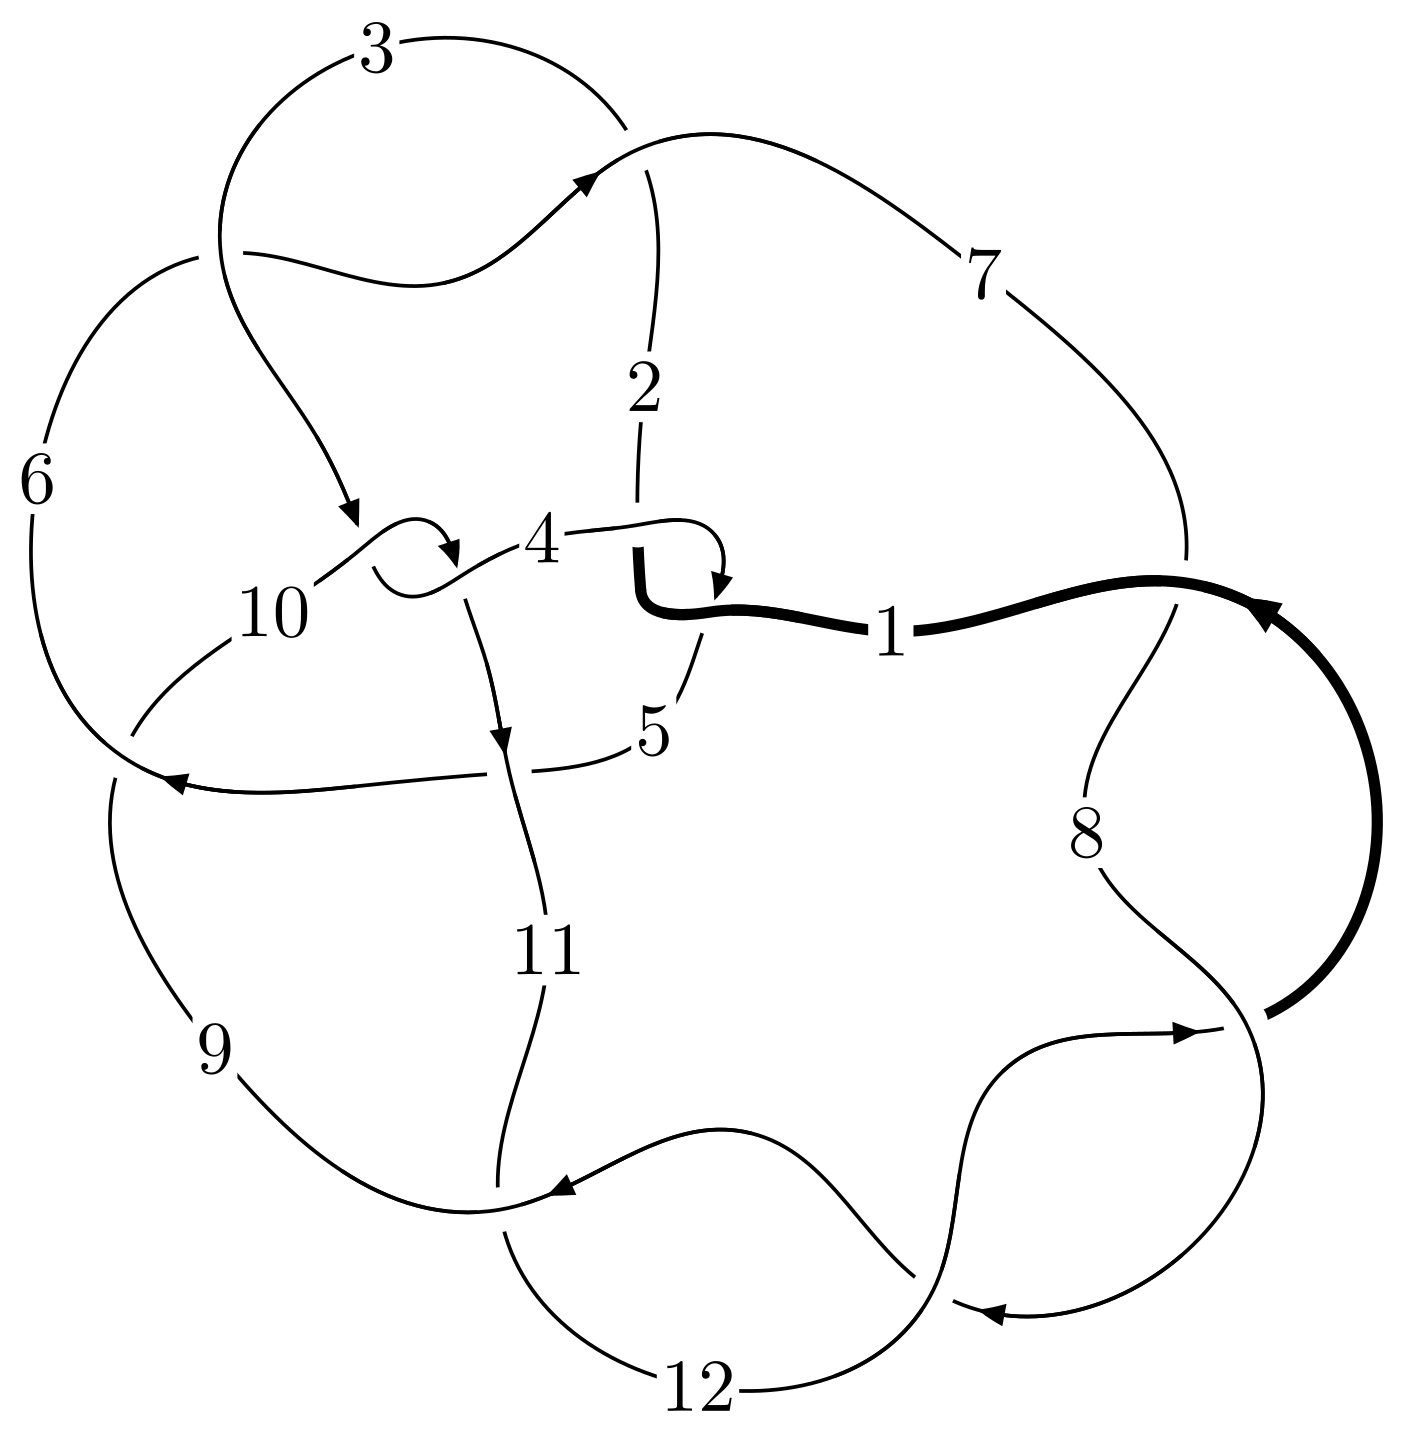
\includegraphics[width=112pt]{../../../GIT/diagram.site/Diagrams/png/2894_12n_0805.png}\\
\ \ \ A knot diagram\footnotemark}&
\allowdisplaybreaks
\textbf{Linearized knot diagam} \\
\cline{2-2}
 &
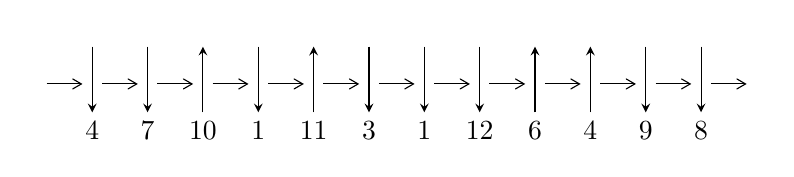
\begin{tikzpicture}[x=20pt, y=17pt]
	% nodes
	\node (C0) at (0, 0) {};
	\node (C1) at (1, 0) {};
	\node (C1U) at (1, +1) {};
	\node (C1D) at (1, -1) {4};

	\node (C2) at (2, 0) {};
	\node (C2U) at (2, +1) {};
	\node (C2D) at (2, -1) {7};

	\node (C3) at (3, 0) {};
	\node (C3U) at (3, +1) {};
	\node (C3D) at (3, -1) {10};

	\node (C4) at (4, 0) {};
	\node (C4U) at (4, +1) {};
	\node (C4D) at (4, -1) {1};

	\node (C5) at (5, 0) {};
	\node (C5U) at (5, +1) {};
	\node (C5D) at (5, -1) {11};

	\node (C6) at (6, 0) {};
	\node (C6U) at (6, +1) {};
	\node (C6D) at (6, -1) {3};

	\node (C7) at (7, 0) {};
	\node (C7U) at (7, +1) {};
	\node (C7D) at (7, -1) {1};

	\node (C8) at (8, 0) {};
	\node (C8U) at (8, +1) {};
	\node (C8D) at (8, -1) {12};

	\node (C9) at (9, 0) {};
	\node (C9U) at (9, +1) {};
	\node (C9D) at (9, -1) {6};

	\node (C10) at (10, 0) {};
	\node (C10U) at (10, +1) {};
	\node (C10D) at (10, -1) {4};

	\node (C11) at (11, 0) {};
	\node (C11U) at (11, +1) {};
	\node (C11D) at (11, -1) {9};

	\node (C12) at (12, 0) {};
	\node (C12U) at (12, +1) {};
	\node (C12D) at (12, -1) {8};
	\node (C13) at (13, 0) {};

	% arrows
	\draw[->,>={angle 60}]
	(C0) edge (C1) (C1) edge (C2) (C2) edge (C3) (C3) edge (C4) (C4) edge (C5) (C5) edge (C6) (C6) edge (C7) (C7) edge (C8) (C8) edge (C9) (C9) edge (C10) (C10) edge (C11) (C11) edge (C12) (C12) edge (C13) ;	\draw[->,>=stealth]
	(C1U) edge (C1D) (C2U) edge (C2D) (C3D) edge (C3U) (C4U) edge (C4D) (C5D) edge (C5U) (C6U) edge (C6D) (C7U) edge (C7D) (C8U) edge (C8D) (C9D) edge (C9U) (C10D) edge (C10U) (C11U) edge (C11D) (C12U) edge (C12D) ;
	\end{tikzpicture} \\
\hhline{~~} \\& 
\textbf{Solving Sequence} \\ \cline{2-2} 
 &
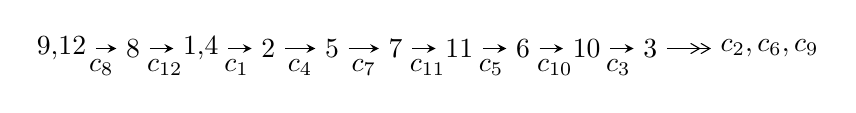
\begin{tikzpicture}[x=23pt, y=7pt]
	% node
	\node (A0) at (-1/8, 0) {9,12};
	\node (A1) at (1, 0) {8};
	\node (A2) at (33/16, 0) {1,4};
	\node (A3) at (25/8, 0) {2};
	\node (A4) at (33/8, 0) {5};
	\node (A5) at (41/8, 0) {7};
	\node (A6) at (49/8, 0) {11};
	\node (A7) at (57/8, 0) {6};
	\node (A8) at (65/8, 0) {10};
	\node (A9) at (73/8, 0) {3};
	\node (C1) at (1/2, -1) {$c_{8}$};
	\node (C2) at (3/2, -1) {$c_{12}$};
	\node (C3) at (21/8, -1) {$c_{1}$};
	\node (C4) at (29/8, -1) {$c_{4}$};
	\node (C5) at (37/8, -1) {$c_{7}$};
	\node (C6) at (45/8, -1) {$c_{11}$};
	\node (C7) at (53/8, -1) {$c_{5}$};
	\node (C8) at (61/8, -1) {$c_{10}$};
	\node (C9) at (69/8, -1) {$c_{3}$};
	\node (A10) at (11, 0) {$c_{2},c_{6},c_{9}$};

	% edge
	\draw[->,>=stealth]	
	(A0) edge (A1) (A1) edge (A2) (A2) edge (A3) (A3) edge (A4) (A4) edge (A5) (A5) edge (A6) (A6) edge (A7) (A7) edge (A8) (A8) edge (A9) ;
	\draw[->>,>={angle 60}]	
	(A9) edge (A10);
\end{tikzpicture} \\ 

\end{tabular} \\

\footnotetext{
The image of knot diagram is generated by the software ``\textbf{Draw programme}" developed by Andrew Bartholomew(\url{http://www.layer8.co.uk/maths/draw/index.htm\#Running-draw}), where we modified some parts for our purpose(\url{https://github.com/CATsTAILs/LinksPainter}).
}\phantom \\ \newline 
\centering \textbf{Ideals for irreducible components\footnotemark of $X_{\text{par}}$} 
 
\begin{align*}
I^u_{1}&=\langle 
-3 u^{21}-14 u^{20}+\cdots+2 b-6,\;-5 u^{21}-28 u^{20}+\cdots+4 a-36,\;u^{22}+6 u^{21}+\cdots+22 u+4\rangle \\
I^u_{2}&=\langle 
-7988 u^7 a^3+5153 u^7 a^2+\cdots-10905 a+11031,\;u^7 a^2+4 u^7 a+\cdots-2 a+7,\\
\phantom{I^u_{2}}&\phantom{= \langle  }u^8- u^7+5 u^6-4 u^5+7 u^4-4 u^3+2 u^2+1\rangle \\
I^u_{3}&=\langle 
- u^{11}+u^{10}-8 u^9+7 u^8-23 u^7+17 u^6-29 u^5+16 u^4-16 u^3+3 u^2+b-3 u-1,\\
\phantom{I^u_{3}}&\phantom{= \langle  }- u^{10}+2 u^9-9 u^8+14 u^7-29 u^6+33 u^5-40 u^4+30 u^3-22 u^2+a+9 u-3,\\
\phantom{I^u_{3}}&\phantom{= \langle  }u^{12}- u^{11}+9 u^{10}-8 u^9+30 u^8-23 u^7+45 u^6-28 u^5+30 u^4-12 u^3+9 u^2+1\rangle \\
\\
\end{align*}
\raggedright * 3 irreducible components of $\dim_{\mathbb{C}}=0$, with total 66 representations.\\
\footnotetext{All coefficients of polynomials are rational numbers. But the coefficients are sometimes approximated in decimal forms when there is not enough margin.}
\newpage
\renewcommand{\arraystretch}{1}
\centering \section*{I. $I^u_{1}= \langle -3 u^{21}-14 u^{20}+\cdots+2 b-6,\;-5 u^{21}-28 u^{20}+\cdots+4 a-36,\;u^{22}+6 u^{21}+\cdots+22 u+4 \rangle$}
\flushleft \textbf{(i) Arc colorings}\\
\begin{tabular}{m{7pt} m{180pt} m{7pt} m{180pt} }
\flushright $a_{9}=$&$\begin{pmatrix}1\\0\end{pmatrix}$ \\
\flushright $a_{12}=$&$\begin{pmatrix}0\\u\end{pmatrix}$ \\
\flushright $a_{8}=$&$\begin{pmatrix}1\\- u^2\end{pmatrix}$ \\
\flushright $a_{1}=$&$\begin{pmatrix}- u\\u^3+u\end{pmatrix}$ \\
\flushright $a_{4}=$&$\begin{pmatrix}\frac{5}{4} u^{21}+7 u^{20}+\cdots+\frac{125}{4} u+9\\\frac{3}{2} u^{21}+7 u^{20}+\cdots+\frac{29}{2} u+3\end{pmatrix}$ \\
\flushright $a_{2}=$&$\begin{pmatrix}-\frac{1}{2} u^{21}-\frac{5}{2} u^{20}+\cdots-\frac{3}{2} u+\frac{5}{2}\\-\frac{1}{2} u^{21}-3 u^{20}+\cdots-20 u^2-\frac{11}{2} u\end{pmatrix}$ \\
\flushright $a_{5}=$&$\begin{pmatrix}\frac{5}{4} u^{21}+7 u^{20}+\cdots+\frac{109}{4} u+7\\\frac{1}{2} u^{21}+4 u^{20}+\cdots+\frac{37}{2} u+5\end{pmatrix}$ \\
\flushright $a_{7}=$&$\begin{pmatrix}u^2+1\\- u^4-2 u^2\end{pmatrix}$ \\
\flushright $a_{11}=$&$\begin{pmatrix}u\\u\end{pmatrix}$ \\
\flushright $a_{6}=$&$\begin{pmatrix}-\frac{3}{4} u^{21}-4 u^{20}+\cdots-\frac{11}{4} u+1\\-\frac{3}{2} u^{21}-7 u^{20}+\cdots-\frac{23}{2} u-1\end{pmatrix}$ \\
\flushright $a_{10}=$&$\begin{pmatrix}-\frac{1}{2} u^{21}-\frac{5}{2} u^{20}+\cdots-\frac{3}{2} u+\frac{1}{2}\\\frac{1}{2} u^{21}+3 u^{20}+\cdots+\frac{37}{2} u+4\end{pmatrix}$ \\
\flushright $a_{3}=$&$\begin{pmatrix}\frac{1}{2} u^{20}+3 u^{19}+\cdots+18 u+\frac{13}{2}\\-\frac{1}{2} u^{21}-2 u^{20}+\cdots-6 u^2-\frac{3}{2} u\end{pmatrix}$\\&\end{tabular}
\flushleft \textbf{(ii) Obstruction class $= -1$}\\~\\
\flushleft \textbf{(iii) Cusp Shapes $= 5 u^{21}+27 u^{20}+137 u^{19}+457 u^{18}+1341 u^{17}+3187 u^{16}+6649 u^{15}+11918 u^{14}+18804 u^{13}+25932 u^{12}+31399 u^{11}+33139 u^{10}+30322 u^9+23720 u^8+15633 u^7+8484 u^6+3756 u^5+1394 u^4+536 u^3+233 u^2+84 u+10$}\\~\\
\newpage\renewcommand{\arraystretch}{1}
\flushleft \textbf{(iv) u-Polynomials at the component}\newline \\
\begin{tabular}{m{50pt}|m{274pt}}
Crossings & \hspace{64pt}u-Polynomials at each crossing \\
\hline $$\begin{aligned}c_{1},c_{4}\end{aligned}$$&$\begin{aligned}
&u^{22}- u^{21}+\cdots-5 u+1
\end{aligned}$\\
\hline $$\begin{aligned}c_{2},c_{6}\end{aligned}$$&$\begin{aligned}
&u^{22}+17 u^{21}+\cdots+2816 u+256
\end{aligned}$\\
\hline $$\begin{aligned}c_{3},c_{9},c_{10}\end{aligned}$$&$\begin{aligned}
&u^{22}- u^{21}+\cdots- u+1
\end{aligned}$\\
\hline $$\begin{aligned}c_{5}\end{aligned}$$&$\begin{aligned}
&u^{22}+4 u^{20}+\cdots-4 u+1
\end{aligned}$\\
\hline $$\begin{aligned}c_{7},c_{8},c_{11}\\c_{12}\end{aligned}$$&$\begin{aligned}
&u^{22}-6 u^{21}+\cdots-22 u+4
\end{aligned}$\\
\hline
\end{tabular}\\~\\
\newpage\renewcommand{\arraystretch}{1}
\flushleft \textbf{(v) Riley Polynomials at the component}\newline \\
\begin{tabular}{m{50pt}|m{274pt}}
Crossings & \hspace{64pt}Riley Polynomials at each crossing \\
\hline $$\begin{aligned}c_{1},c_{4}\end{aligned}$$&$\begin{aligned}
&y^{22}-23 y^{21}+\cdots+13 y+1
\end{aligned}$\\
\hline $$\begin{aligned}c_{2},c_{6}\end{aligned}$$&$\begin{aligned}
&y^{22}+9 y^{21}+\cdots+393216 y+65536
\end{aligned}$\\
\hline $$\begin{aligned}c_{3},c_{9},c_{10}\end{aligned}$$&$\begin{aligned}
&y^{22}-13 y^{21}+\cdots- y+1
\end{aligned}$\\
\hline $$\begin{aligned}c_{5}\end{aligned}$$&$\begin{aligned}
&y^{22}+8 y^{21}+\cdots+12 y+1
\end{aligned}$\\
\hline $$\begin{aligned}c_{7},c_{8},c_{11}\\c_{12}\end{aligned}$$&$\begin{aligned}
&y^{22}+26 y^{21}+\cdots+36 y+16
\end{aligned}$\\
\hline
\end{tabular}\\~\\
\newpage\flushleft \textbf{(vi) Complex Volumes and Cusp Shapes}
$$\begin{array}{c|c|c}  
\text{Solutions to }I^u_{1}& \I (\text{vol} + \sqrt{-1}CS) & \text{Cusp shape}\\
 \hline 
\begin{aligned}
u &= -0.672231 + 0.669430 I \\
a &= -0.646053 + 0.197647 I \\
b &= -1.12221 - 1.29155 I\end{aligned}
 & \phantom{-}1.57285 + 10.92870 I & -0.09523 - 8.13846 I \\ \hline\begin{aligned}
u &= -0.672231 - 0.669430 I \\
a &= -0.646053 - 0.197647 I \\
b &= -1.12221 + 1.29155 I\end{aligned}
 & \phantom{-}1.57285 - 10.92870 I & -0.09523 + 8.13846 I \\ \hline\begin{aligned}
u &= -0.535508 + 0.711181 I \\
a &= \phantom{-}0.314853 + 0.241466 I \\
b &= \phantom{-}0.606532 + 1.248090 I\end{aligned}
 & -1.54704 + 3.14824 I & \phantom{-}0.77612 - 6.02980 I \\ \hline\begin{aligned}
u &= -0.535508 - 0.711181 I \\
a &= \phantom{-}0.314853 - 0.241466 I \\
b &= \phantom{-}0.606532 - 1.248090 I\end{aligned}
 & -1.54704 - 3.14824 I & \phantom{-}0.77612 + 6.02980 I \\ \hline\begin{aligned}
u &= -0.759597 + 0.320799 I \\
a &= -1.058800 - 0.555950 I \\
b &= \phantom{-}0.598202 - 0.762166 I\end{aligned}
 & \phantom{-}0.54148 - 6.16925 I & -2.10987 + 3.70957 I \\ \hline\begin{aligned}
u &= -0.759597 - 0.320799 I \\
a &= -1.058800 + 0.555950 I \\
b &= \phantom{-}0.598202 + 0.762166 I\end{aligned}
 & \phantom{-}0.54148 + 6.16925 I & -2.10987 - 3.70957 I \\ \hline\begin{aligned}
u &= -0.288943 + 1.232890 I \\
a &= \phantom{-}0.412257 + 0.459691 I \\
b &= -0.222633 - 0.193104 I\end{aligned}
 & \phantom{-}5.51465 - 2.42737 I & \phantom{-}0.51879 + 3.32610 I \\ \hline\begin{aligned}
u &= -0.288943 - 1.232890 I \\
a &= \phantom{-}0.412257 - 0.459691 I \\
b &= -0.222633 + 0.193104 I\end{aligned}
 & \phantom{-}5.51465 + 2.42737 I & \phantom{-}0.51879 - 3.32610 I \\ \hline\begin{aligned}
u &= \phantom{-}0.068378 + 1.330140 I \\
a &= \phantom{-}0.746060 - 0.076338 I \\
b &= \phantom{-}0.327439 - 0.582001 I\end{aligned}
 & \phantom{-}5.16986 - 2.20242 I & \phantom{-}0.58597 + 3.53079 I \\ \hline\begin{aligned}
u &= \phantom{-}0.068378 - 1.330140 I \\
a &= \phantom{-}0.746060 + 0.076338 I \\
b &= \phantom{-}0.327439 + 0.582001 I\end{aligned}
 & \phantom{-}5.16986 + 2.20242 I & \phantom{-}0.58597 - 3.53079 I\\
 \hline 
 \end{array}$$\newpage$$\begin{array}{c|c|c}  
\text{Solutions to }I^u_{1}& \I (\text{vol} + \sqrt{-1}CS) & \text{Cusp shape}\\
 \hline 
\begin{aligned}
u &= -0.540881 + 0.284720 I \\
a &= \phantom{-}1.42566 + 0.38957 I \\
b &= \phantom{-}0.256071 + 0.621077 I\end{aligned}
 & -2.84705 + 0.58927 I & -4.02070 + 2.06270 I \\ \hline\begin{aligned}
u &= -0.540881 - 0.284720 I \\
a &= \phantom{-}1.42566 - 0.38957 I \\
b &= \phantom{-}0.256071 - 0.621077 I\end{aligned}
 & -2.84705 - 0.58927 I & -4.02070 - 2.06270 I \\ \hline\begin{aligned}
u &= -0.11745 + 1.45301 I \\
a &= -1.65572 - 0.36277 I \\
b &= -1.100210 - 0.121955 I\end{aligned}
 & \phantom{-}2.80552 + 2.73021 I & -1.72854 - 0.56419 I \\ \hline\begin{aligned}
u &= -0.11745 - 1.45301 I \\
a &= -1.65572 + 0.36277 I \\
b &= -1.100210 + 0.121955 I\end{aligned}
 & \phantom{-}2.80552 - 2.73021 I & -1.72854 + 0.56419 I \\ \hline\begin{aligned}
u &= \phantom{-}0.276614 + 0.310933 I \\
a &= -0.535008 - 0.626026 I \\
b &= -0.121326 + 0.413923 I\end{aligned}
 & -0.116282 - 0.855526 I & -2.84227 + 8.01769 I \\ \hline\begin{aligned}
u &= \phantom{-}0.276614 - 0.310933 I \\
a &= -0.535008 + 0.626026 I \\
b &= -0.121326 - 0.413923 I\end{aligned}
 & -0.116282 + 0.855526 I & -2.84227 - 8.01769 I \\ \hline\begin{aligned}
u &= -0.21959 + 1.59057 I \\
a &= \phantom{-}1.99989 + 0.71251 I \\
b &= \phantom{-}1.71567 + 1.64082 I\end{aligned}
 & \phantom{-}9.0925 + 14.2705 I & \phantom{-}2.92033 - 7.26786 I \\ \hline\begin{aligned}
u &= -0.21959 - 1.59057 I \\
a &= \phantom{-}1.99989 - 0.71251 I \\
b &= \phantom{-}1.71567 - 1.64082 I\end{aligned}
 & \phantom{-}9.0925 - 14.2705 I & \phantom{-}2.92033 + 7.26786 I \\ \hline\begin{aligned}
u &= -0.17706 + 1.62106 I \\
a &= -1.41137 - 1.11105 I \\
b &= -1.29958 - 1.77102 I\end{aligned}
 & \phantom{-}6.38360 + 5.88492 I & \phantom{-}3.26398 - 4.41155 I \\ \hline\begin{aligned}
u &= -0.17706 - 1.62106 I \\
a &= -1.41137 + 1.11105 I \\
b &= -1.29958 + 1.77102 I\end{aligned}
 & \phantom{-}6.38360 - 5.88492 I & \phantom{-}3.26398 + 4.41155 I\\
 \hline 
 \end{array}$$\newpage$$\begin{array}{c|c|c}  
\text{Solutions to }I^u_{1}& \I (\text{vol} + \sqrt{-1}CS) & \text{Cusp shape}\\
 \hline 
\begin{aligned}
u &= -0.03373 + 1.75344 I \\
a &= \phantom{-}0.158232 + 0.724477 I \\
b &= \phantom{-}0.362036 + 1.269890 I\end{aligned}
 & \phantom{-}16.1982 - 1.4224 I & -2.26858 + 6.72406 I \\ \hline\begin{aligned}
u &= -0.03373 - 1.75344 I \\
a &= \phantom{-}0.158232 - 0.724477 I \\
b &= \phantom{-}0.362036 - 1.269890 I\end{aligned}
 & \phantom{-}16.1982 + 1.4224 I & -2.26858 - 6.72406 I\\
 \hline 
 \end{array}$$\newpage\newpage\renewcommand{\arraystretch}{1}
\centering \section*{II. $I^u_{2}= \langle -7988 u^7 a^3+5153 u^7 a^2+\cdots-10905 a+11031,\;u^7 a^2+4 u^7 a+\cdots-2 a+7,\;u^8- u^7+5 u^6-4 u^5+7 u^4-4 u^3+2 u^2+1 \rangle$}
\flushleft \textbf{(i) Arc colorings}\\
\begin{tabular}{m{7pt} m{180pt} m{7pt} m{180pt} }
\flushright $a_{9}=$&$\begin{pmatrix}1\\0\end{pmatrix}$ \\
\flushright $a_{12}=$&$\begin{pmatrix}0\\u\end{pmatrix}$ \\
\flushright $a_{8}=$&$\begin{pmatrix}1\\- u^2\end{pmatrix}$ \\
\flushright $a_{1}=$&$\begin{pmatrix}- u\\u^3+u\end{pmatrix}$ \\
\flushright $a_{4}=$&$\begin{pmatrix}a\\0.148683 a^{3} u^{7}-0.0959144 a^{2} u^{7}+\cdots+0.202978 a-0.205323\end{pmatrix}$ \\
\flushright $a_{2}=$&$\begin{pmatrix}0.368581 a^{3} u^{7}+0.700102 a^{2} u^{7}+\cdots-0.361657 a-0.327110\\0.140679 a^{3} u^{7}+0.558902 a^{2} u^{7}+\cdots-0.629502 a+0.738092\end{pmatrix}$ \\
\flushright $a_{5}=$&$\begin{pmatrix}-0.136194 a^{3} u^{7}+0.0847278 a^{2} u^{7}+\cdots+1.22531 a+0.554751\\0.227231 a^{3} u^{7}-0.0604560 a^{2} u^{7}+\cdots+1.39283 a-0.244691\end{pmatrix}$ \\
\flushright $a_{7}=$&$\begin{pmatrix}u^2+1\\- u^4-2 u^2\end{pmatrix}$ \\
\flushright $a_{11}=$&$\begin{pmatrix}u\\u\end{pmatrix}$ \\
\flushright $a_{6}=$&$\begin{pmatrix}-0.725305 a^{3} u^{7}-0.681210 a^{2} u^{7}+\cdots+0.801396 a+0.350005\\-0.361880 a^{3} u^{7}-0.826394 a^{2} u^{7}+\cdots+0.968916 a-0.449437\end{pmatrix}$ \\
\flushright $a_{10}=$&$\begin{pmatrix}-0.368581 a^{3} u^{7}-0.700102 a^{2} u^{7}+\cdots+0.361657 a+0.327110\\0.0635458 a^{3} u^{7}-0.209567 a^{2} u^{7}+\cdots+0.980270 a-0.811875\end{pmatrix}$ \\
\flushright $a_{3}=$&$\begin{pmatrix}-0.463993 a^{3} u^{7}+0.141796 a^{2} u^{7}+\cdots-0.563611 a+0.158883\\-0.312611 a^{3} u^{7}-0.467287 a^{2} u^{7}+\cdots+0.616101 a+1.29158\end{pmatrix}$\\&\end{tabular}
\flushleft \textbf{(ii) Obstruction class $= -1$}\\~\\
\flushleft \textbf{(iii) Cusp Shapes $= -\frac{6416}{7675} u^7 a^3-\frac{10404}{7675} u^7 a^2+\cdots+\frac{4668}{1535} a+\frac{12542}{7675}$}\\~\\
\newpage\renewcommand{\arraystretch}{1}
\flushleft \textbf{(iv) u-Polynomials at the component}\newline \\
\begin{tabular}{m{50pt}|m{274pt}}
Crossings & \hspace{64pt}u-Polynomials at each crossing \\
\hline $$\begin{aligned}c_{1},c_{4}\end{aligned}$$&$\begin{aligned}
&u^{32}-7 u^{31}+\cdots-110 u+37
\end{aligned}$\\
\hline $$\begin{aligned}c_{2},c_{6}\end{aligned}$$&$\begin{aligned}
&(u^2- u+1)^{16}
\end{aligned}$\\
\hline $$\begin{aligned}c_{3},c_{9},c_{10}\end{aligned}$$&$\begin{aligned}
&u^{32}+u^{31}+\cdots+300 u+343
\end{aligned}$\\
\hline $$\begin{aligned}c_{5}\end{aligned}$$&$\begin{aligned}
&u^{32}+u^{31}+\cdots-2776 u+343
\end{aligned}$\\
\hline $$\begin{aligned}c_{7},c_{8},c_{11}\\c_{12}\end{aligned}$$&$\begin{aligned}
&(u^8+u^7+5 u^6+4 u^5+7 u^4+4 u^3+2 u^2+1)^4
\end{aligned}$\\
\hline
\end{tabular}\\~\\
\newpage\renewcommand{\arraystretch}{1}
\flushleft \textbf{(v) Riley Polynomials at the component}\newline \\
\begin{tabular}{m{50pt}|m{274pt}}
Crossings & \hspace{64pt}Riley Polynomials at each crossing \\
\hline $$\begin{aligned}c_{1},c_{4}\end{aligned}$$&$\begin{aligned}
&y^{32}-5 y^{31}+\cdots-28528 y+1369
\end{aligned}$\\
\hline $$\begin{aligned}c_{2},c_{6}\end{aligned}$$&$\begin{aligned}
&(y^2+y+1)^{16}
\end{aligned}$\\
\hline $$\begin{aligned}c_{3},c_{9},c_{10}\end{aligned}$$&$\begin{aligned}
&y^{32}-21 y^{31}+\cdots-1386540 y+117649
\end{aligned}$\\
\hline $$\begin{aligned}c_{5}\end{aligned}$$&$\begin{aligned}
&y^{32}-13 y^{31}+\cdots-8932744 y+117649
\end{aligned}$\\
\hline $$\begin{aligned}c_{7},c_{8},c_{11}\\c_{12}\end{aligned}$$&$\begin{aligned}
&(y^8+9 y^7+31 y^6+50 y^5+39 y^4+22 y^3+18 y^2+4 y+1)^4
\end{aligned}$\\
\hline
\end{tabular}\\~\\
\newpage\flushleft \textbf{(vi) Complex Volumes and Cusp Shapes}
$$\begin{array}{c|c|c}  
\text{Solutions to }I^u_{2}& \I (\text{vol} + \sqrt{-1}CS) & \text{Cusp shape}\\
 \hline 
\begin{aligned}
u &= \phantom{-}0.647085 + 0.502738 I \\
a &= \phantom{-}0.592287 - 0.833358 I \\
b &= -0.453639 - 0.557953 I\end{aligned}
 & -1.67479 - 0.15547 I & -1.58319 - 0.32355 I \\ \hline\begin{aligned}
u &= \phantom{-}0.647085 + 0.502738 I \\
a &= -1.270790 + 0.209688 I \\
b &= -0.057820 + 1.153500 I\end{aligned}
 & -1.67479 - 4.21524 I & -1.58319 + 6.60465 I \\ \hline\begin{aligned}
u &= \phantom{-}0.647085 + 0.502738 I \\
a &= -0.630581 - 0.097668 I \\
b &= -0.355056 + 1.312410 I\end{aligned}
 & -1.67479 - 0.15547 I & -1.58319 - 0.32355 I \\ \hline\begin{aligned}
u &= \phantom{-}0.647085 + 0.502738 I \\
a &= \phantom{-}0.483643 + 0.288989 I \\
b &= \phantom{-}1.115550 - 0.830375 I\end{aligned}
 & -1.67479 - 4.21524 I & -1.58319 + 6.60465 I \\ \hline\begin{aligned}
u &= \phantom{-}0.647085 - 0.502738 I \\
a &= \phantom{-}0.592287 + 0.833358 I \\
b &= -0.453639 + 0.557953 I\end{aligned}
 & -1.67479 + 0.15547 I & -1.58319 + 0.32355 I \\ \hline\begin{aligned}
u &= \phantom{-}0.647085 - 0.502738 I \\
a &= -1.270790 - 0.209688 I \\
b &= -0.057820 - 1.153500 I\end{aligned}
 & -1.67479 + 4.21524 I & -1.58319 - 6.60465 I \\ \hline\begin{aligned}
u &= \phantom{-}0.647085 - 0.502738 I \\
a &= -0.630581 + 0.097668 I \\
b &= -0.355056 - 1.312410 I\end{aligned}
 & -1.67479 + 0.15547 I & -1.58319 + 0.32355 I \\ \hline\begin{aligned}
u &= \phantom{-}0.647085 - 0.502738 I \\
a &= \phantom{-}0.483643 - 0.288989 I \\
b &= \phantom{-}1.115550 + 0.830375 I\end{aligned}
 & -1.67479 + 4.21524 I & -1.58319 - 6.60465 I \\ \hline\begin{aligned}
u &= -0.283060 + 0.443755 I \\
a &= \phantom{-}0.498434 + 1.041700 I \\
b &= -0.57514 - 1.33218 I\end{aligned}
 & \phantom{-}4.93480 + 3.07589 I & \phantom{-}2.00000 - 10.14955 I \\ \hline\begin{aligned}
u &= -0.283060 + 0.443755 I \\
a &= -0.537114 + 1.186060 I \\
b &= -1.91169 - 0.11910 I\end{aligned}
 & \phantom{-}4.93480 - 0.98388 I & \phantom{-}2.00000 - 3.22135 I\\
 \hline 
 \end{array}$$\newpage$$\begin{array}{c|c|c}  
\text{Solutions to }I^u_{2}& \I (\text{vol} + \sqrt{-1}CS) & \text{Cusp shape}\\
 \hline 
\begin{aligned}
u &= -0.283060 + 0.443755 I \\
a &= -1.55933 - 2.06959 I \\
b &= \phantom{-}0.389762 + 0.054060 I\end{aligned}
 & \phantom{-}4.93480 - 0.98388 I & \phantom{-}2.00000 - 3.22135 I \\ \hline\begin{aligned}
u &= -0.283060 + 0.443755 I \\
a &= \phantom{-}1.31495 - 2.41550 I \\
b &= \phantom{-}1.392430 + 0.046674 I\end{aligned}
 & \phantom{-}4.93480 + 3.07589 I & \phantom{-}2.00000 - 10.14955 I \\ \hline\begin{aligned}
u &= -0.283060 - 0.443755 I \\
a &= \phantom{-}0.498434 - 1.041700 I \\
b &= -0.57514 + 1.33218 I\end{aligned}
 & \phantom{-}4.93480 - 3.07589 I & \phantom{-}2.00000 + 10.14955 I \\ \hline\begin{aligned}
u &= -0.283060 - 0.443755 I \\
a &= -0.537114 - 1.186060 I \\
b &= -1.91169 + 0.11910 I\end{aligned}
 & \phantom{-}4.93480 + 0.98388 I & \phantom{-}2.00000 + 3.22135 I \\ \hline\begin{aligned}
u &= -0.283060 - 0.443755 I \\
a &= -1.55933 + 2.06959 I \\
b &= \phantom{-}0.389762 - 0.054060 I\end{aligned}
 & \phantom{-}4.93480 + 0.98388 I & \phantom{-}2.00000 + 3.22135 I \\ \hline\begin{aligned}
u &= -0.283060 - 0.443755 I \\
a &= \phantom{-}1.31495 + 2.41550 I \\
b &= \phantom{-}1.392430 - 0.046674 I\end{aligned}
 & \phantom{-}4.93480 - 3.07589 I & \phantom{-}2.00000 + 10.14955 I \\ \hline\begin{aligned}
u &= -0.06382 + 1.51723 I \\
a &= -0.112835 + 0.153959 I \\
b &= -0.343676 - 0.971058 I\end{aligned}
 & \phantom{-}11.54440 + 0.15547 I & \phantom{-}5.58319 + 0.32355 I \\ \hline\begin{aligned}
u &= -0.06382 + 1.51723 I \\
a &= \phantom{-}0.82329 + 1.83665 I \\
b &= \phantom{-}0.76874 + 2.76112 I\end{aligned}
 & \phantom{-}11.54440 + 4.21524 I & \phantom{-}5.58319 - 6.60465 I \\ \hline\begin{aligned}
u &= -0.06382 + 1.51723 I \\
a &= -2.24271 + 0.60948 I \\
b &= -1.65098 - 0.26388 I\end{aligned}
 & \phantom{-}11.54440 + 4.21524 I & \phantom{-}5.58319 - 6.60465 I \\ \hline\begin{aligned}
u &= -0.06382 + 1.51723 I \\
a &= \phantom{-}2.94096 - 0.14777 I \\
b &= \phantom{-}2.94748 + 0.48648 I\end{aligned}
 & \phantom{-}11.54440 + 0.15547 I & \phantom{-}5.58319 + 0.32355 I\\
 \hline 
 \end{array}$$\newpage$$\begin{array}{c|c|c}  
\text{Solutions to }I^u_{2}& \I (\text{vol} + \sqrt{-1}CS) & \text{Cusp shape}\\
 \hline 
\begin{aligned}
u &= -0.06382 - 1.51723 I \\
a &= -0.112835 - 0.153959 I \\
b &= -0.343676 + 0.971058 I\end{aligned}
 & \phantom{-}11.54440 - 0.15547 I & \phantom{-}5.58319 - 0.32355 I \\ \hline\begin{aligned}
u &= -0.06382 - 1.51723 I \\
a &= \phantom{-}0.82329 - 1.83665 I \\
b &= \phantom{-}0.76874 - 2.76112 I\end{aligned}
 & \phantom{-}11.54440 - 4.21524 I & \phantom{-}5.58319 + 6.60465 I \\ \hline\begin{aligned}
u &= -0.06382 - 1.51723 I \\
a &= -2.24271 - 0.60948 I \\
b &= -1.65098 + 0.26388 I\end{aligned}
 & \phantom{-}11.54440 - 4.21524 I & \phantom{-}5.58319 + 6.60465 I \\ \hline\begin{aligned}
u &= -0.06382 - 1.51723 I \\
a &= \phantom{-}2.94096 + 0.14777 I \\
b &= \phantom{-}2.94748 - 0.48648 I\end{aligned}
 & \phantom{-}11.54440 - 0.15547 I & \phantom{-}5.58319 - 0.32355 I \\ \hline\begin{aligned}
u &= \phantom{-}0.19980 + 1.51366 I \\
a &= -0.413833 + 0.373606 I \\
b &= -0.166931 + 0.023712 I\end{aligned}
 & \phantom{-}4.93480 - 3.20880 I & \phantom{-}2.00000 - 0.42152 I \\ \hline\begin{aligned}
u &= \phantom{-}0.19980 + 1.51366 I \\
a &= \phantom{-}1.37518 - 0.69793 I \\
b &= \phantom{-}0.87012 - 1.31414 I\end{aligned}
 & \phantom{-}4.93480 - 3.20880 I & \phantom{-}2.00000 - 0.42152 I \\ \hline\begin{aligned}
u &= \phantom{-}0.19980 + 1.51366 I \\
a &= \phantom{-}1.34760 - 0.78701 I \\
b &= \phantom{-}0.439335 - 0.833174 I\end{aligned}
 & \phantom{-}4.93480 - 7.26857 I & \phantom{-}2.00000 + 6.50668 I \\ \hline\begin{aligned}
u &= \phantom{-}0.19980 + 1.51366 I \\
a &= -2.10915 + 0.11662 I \\
b &= -1.90847 + 0.86941 I\end{aligned}
 & \phantom{-}4.93480 - 7.26857 I & \phantom{-}2.00000 + 6.50668 I \\ \hline\begin{aligned}
u &= \phantom{-}0.19980 - 1.51366 I \\
a &= -0.413833 - 0.373606 I \\
b &= -0.166931 - 0.023712 I\end{aligned}
 & \phantom{-}4.93480 + 3.20880 I & \phantom{-}2.00000 + 0.42152 I \\ \hline\begin{aligned}
u &= \phantom{-}0.19980 - 1.51366 I \\
a &= \phantom{-}1.37518 + 0.69793 I \\
b &= \phantom{-}0.87012 + 1.31414 I\end{aligned}
 & \phantom{-}4.93480 + 3.20880 I & \phantom{-}2.00000 + 0.42152 I\\
 \hline 
 \end{array}$$\newpage$$\begin{array}{c|c|c}  
\text{Solutions to }I^u_{2}& \I (\text{vol} + \sqrt{-1}CS) & \text{Cusp shape}\\
 \hline 
\begin{aligned}
u &= \phantom{-}0.19980 - 1.51366 I \\
a &= \phantom{-}1.34760 + 0.78701 I \\
b &= \phantom{-}0.439335 + 0.833174 I\end{aligned}
 & \phantom{-}4.93480 + 7.26857 I & \phantom{-}2.00000 - 6.50668 I \\ \hline\begin{aligned}
u &= \phantom{-}0.19980 - 1.51366 I \\
a &= -2.10915 - 0.11662 I \\
b &= -1.90847 - 0.86941 I\end{aligned}
 & \phantom{-}4.93480 + 7.26857 I & \phantom{-}2.00000 - 6.50668 I\\
 \hline 
 \end{array}$$\newpage\newpage\renewcommand{\arraystretch}{1}
\centering \section*{III. $I^u_{3}= \langle - u^{11}+u^{10}+\cdots+b-1,\;- u^{10}+2 u^9+\cdots+a-3,\;u^{12}- u^{11}+\cdots+9 u^2+1 \rangle$}
\flushleft \textbf{(i) Arc colorings}\\
\begin{tabular}{m{7pt} m{180pt} m{7pt} m{180pt} }
\flushright $a_{9}=$&$\begin{pmatrix}1\\0\end{pmatrix}$ \\
\flushright $a_{12}=$&$\begin{pmatrix}0\\u\end{pmatrix}$ \\
\flushright $a_{8}=$&$\begin{pmatrix}1\\- u^2\end{pmatrix}$ \\
\flushright $a_{1}=$&$\begin{pmatrix}- u\\u^3+u\end{pmatrix}$ \\
\flushright $a_{4}=$&$\begin{pmatrix}u^{10}-2 u^9+9 u^8-14 u^7+29 u^6-33 u^5+40 u^4-30 u^3+22 u^2-9 u+3\\u^{11}- u^{10}+\cdots+3 u+1\end{pmatrix}$ \\
\flushright $a_{2}=$&$\begin{pmatrix}- u^{11}+u^{10}-8 u^9+6 u^8-22 u^7+11 u^6-23 u^5+5 u^4-6 u^3-4 u^2-4\\- u^{11}+2 u^{10}+\cdots-4 u+1\end{pmatrix}$ \\
\flushright $a_{5}=$&$\begin{pmatrix}- u^9+2 u^8-8 u^7+13 u^6-22 u^5+27 u^4-24 u^3+19 u^2-9 u+3\\u^{11}-2 u^{10}+\cdots-9 u^2+3 u\end{pmatrix}$ \\
\flushright $a_{7}=$&$\begin{pmatrix}u^2+1\\- u^4-2 u^2\end{pmatrix}$ \\
\flushright $a_{11}=$&$\begin{pmatrix}u\\u\end{pmatrix}$ \\
\flushright $a_{6}=$&$\begin{pmatrix}u^{10}-2 u^9+\cdots-10 u+4\\u^{11}- u^{10}+\cdots+2 u+1\end{pmatrix}$ \\
\flushright $a_{10}=$&$\begin{pmatrix}u^{11}- u^{10}+\cdots+12 u-4\\- u^9+u^8-7 u^7+6 u^6-16 u^5+11 u^4-13 u^3+6 u^2-3 u-1\end{pmatrix}$ \\
\flushright $a_{3}=$&$\begin{pmatrix}- u^{11}-7 u^9- u^8-16 u^7-6 u^6-11 u^5-12 u^4+3 u^3-11 u^2+2 u-5\\- u^{11}+u^{10}+\cdots+6 u^2-4 u\end{pmatrix}$\\&\end{tabular}
\flushleft \textbf{(ii) Obstruction class $= 1$}\\~\\
\flushleft \textbf{(iii) Cusp Shapes $= 3 u^8+17 u^6- u^5+29 u^4-3 u^3+14 u^2-2 u+7$}\\~\\
\newpage\renewcommand{\arraystretch}{1}
\flushleft \textbf{(iv) u-Polynomials at the component}\newline \\
\begin{tabular}{m{50pt}|m{274pt}}
Crossings & \hspace{64pt}u-Polynomials at each crossing \\
\hline $$\begin{aligned}c_{1}\end{aligned}$$&$\begin{aligned}
&u^{12}- u^{11}-4 u^9+6 u^8-2 u^7+6 u^6-9 u^5+3 u^4-4 u^3+4 u^2+1
\end{aligned}$\\
\hline $$\begin{aligned}c_{2}\end{aligned}$$&$\begin{aligned}
&u^{12}+4 u^{10}-4 u^9+3 u^8-9 u^7+6 u^6-2 u^5+6 u^4-4 u^3- u+1
\end{aligned}$\\
\hline $$\begin{aligned}c_{3},c_{9}\end{aligned}$$&$\begin{aligned}
&u^{12}+u^{11}-5 u^{10}-5 u^9+10 u^8+10 u^7-8 u^6-9 u^5+u^4+3 u^3+u^2+1
\end{aligned}$\\
\hline $$\begin{aligned}c_{4}\end{aligned}$$&$\begin{aligned}
&u^{12}+u^{11}+4 u^9+6 u^8+2 u^7+6 u^6+9 u^5+3 u^4+4 u^3+4 u^2+1
\end{aligned}$\\
\hline $$\begin{aligned}c_{5}\end{aligned}$$&$\begin{aligned}
&u^{12}- u^{10}+\cdots+15 u+37
\end{aligned}$\\
\hline $$\begin{aligned}c_{6}\end{aligned}$$&$\begin{aligned}
&u^{12}+4 u^{10}+4 u^9+3 u^8+9 u^7+6 u^6+2 u^5+6 u^4+4 u^3+u+1
\end{aligned}$\\
\hline $$\begin{aligned}c_{7},c_{8}\end{aligned}$$&$\begin{aligned}
&u^{12}- u^{11}+\cdots+9 u^2+1
\end{aligned}$\\
\hline $$\begin{aligned}c_{10}\end{aligned}$$&$\begin{aligned}
&u^{12}- u^{11}-5 u^{10}+5 u^9+10 u^8-10 u^7-8 u^6+9 u^5+u^4-3 u^3+u^2+1
\end{aligned}$\\
\hline $$\begin{aligned}c_{11},c_{12}\end{aligned}$$&$\begin{aligned}
&u^{12}+u^{11}+\cdots+9 u^2+1
\end{aligned}$\\
\hline
\end{tabular}\\~\\
\newpage\renewcommand{\arraystretch}{1}
\flushleft \textbf{(v) Riley Polynomials at the component}\newline \\
\begin{tabular}{m{50pt}|m{274pt}}
Crossings & \hspace{64pt}Riley Polynomials at each crossing \\
\hline $$\begin{aligned}c_{1},c_{4}\end{aligned}$$&$\begin{aligned}
&y^{12}- y^{11}+\cdots+8 y+1
\end{aligned}$\\
\hline $$\begin{aligned}c_{2},c_{6}\end{aligned}$$&$\begin{aligned}
&y^{12}+8 y^{11}+\cdots- y+1
\end{aligned}$\\
\hline $$\begin{aligned}c_{3},c_{9},c_{10}\end{aligned}$$&$\begin{aligned}
&y^{12}-11 y^{11}+\cdots+2 y+1
\end{aligned}$\\
\hline $$\begin{aligned}c_{5}\end{aligned}$$&$\begin{aligned}
&y^{12}-2 y^{11}+\cdots-373 y+1369
\end{aligned}$\\
\hline $$\begin{aligned}c_{7},c_{8},c_{11}\\c_{12}\end{aligned}$$&$\begin{aligned}
&y^{12}+17 y^{11}+\cdots+18 y+1
\end{aligned}$\\
\hline
\end{tabular}\\~\\
\newpage\flushleft \textbf{(vi) Complex Volumes and Cusp Shapes}
$$\begin{array}{c|c|c}  
\text{Solutions to }I^u_{3}& \I (\text{vol} + \sqrt{-1}CS) & \text{Cusp shape}\\
 \hline 
\begin{aligned}
u &= -0.089013 + 0.906809 I \\
a &= -0.411424 + 0.831833 I \\
b &= -0.881210 - 0.394305 I\end{aligned}
 & \phantom{-}7.14530 - 1.50712 I & \phantom{-}6.80370 + 0.78584 I \\ \hline\begin{aligned}
u &= -0.089013 - 0.906809 I \\
a &= -0.411424 - 0.831833 I \\
b &= -0.881210 + 0.394305 I\end{aligned}
 & \phantom{-}7.14530 + 1.50712 I & \phantom{-}6.80370 - 0.78584 I \\ \hline\begin{aligned}
u &= \phantom{-}0.560380 + 0.536459 I \\
a &= -0.646516 + 0.336204 I \\
b &= -0.397396 + 0.941015 I\end{aligned}
 & -2.38168 - 1.90999 I & -3.16998 + 3.64025 I \\ \hline\begin{aligned}
u &= \phantom{-}0.560380 - 0.536459 I \\
a &= -0.646516 - 0.336204 I \\
b &= -0.397396 - 0.941015 I\end{aligned}
 & -2.38168 + 1.90999 I & -3.16998 - 3.64025 I \\ \hline\begin{aligned}
u &= -0.03756 + 1.51189 I \\
a &= -1.91798 - 0.42547 I \\
b &= -1.68049 - 1.38079 I\end{aligned}
 & \phantom{-}11.54940 + 2.73635 I & \phantom{-}5.59363 - 1.06316 I \\ \hline\begin{aligned}
u &= -0.03756 - 1.51189 I \\
a &= -1.91798 + 0.42547 I \\
b &= -1.68049 + 1.38079 I\end{aligned}
 & \phantom{-}11.54940 - 2.73635 I & \phantom{-}5.59363 + 1.06316 I \\ \hline\begin{aligned}
u &= \phantom{-}0.19341 + 1.55032 I \\
a &= \phantom{-}1.29683 - 0.61636 I \\
b &= \phantom{-}0.971343 - 0.961955 I\end{aligned}
 & \phantom{-}4.61882 - 4.69602 I & \phantom{-}0.54451 + 4.43635 I \\ \hline\begin{aligned}
u &= \phantom{-}0.19341 - 1.55032 I \\
a &= \phantom{-}1.29683 + 0.61636 I \\
b &= \phantom{-}0.971343 + 0.961955 I\end{aligned}
 & \phantom{-}4.61882 + 4.69602 I & \phantom{-}0.54451 - 4.43635 I \\ \hline\begin{aligned}
u &= -0.106406 + 0.331105 I \\
a &= \phantom{-}1.14337 - 3.27977 I \\
b &= \phantom{-}1.29750 + 0.61995 I\end{aligned}
 & \phantom{-}5.16484 + 2.20517 I & \phantom{-}5.88472 - 1.20023 I \\ \hline\begin{aligned}
u &= -0.106406 - 0.331105 I \\
a &= \phantom{-}1.14337 + 3.27977 I \\
b &= \phantom{-}1.29750 - 0.61995 I\end{aligned}
 & \phantom{-}5.16484 - 2.20517 I & \phantom{-}5.88472 + 1.20023 I\\
 \hline 
 \end{array}$$\newpage$$\begin{array}{c|c|c}  
\text{Solutions to }I^u_{3}& \I (\text{vol} + \sqrt{-1}CS) & \text{Cusp shape}\\
 \hline 
\begin{aligned}
u &= -0.02080 + 1.72148 I \\
a &= \phantom{-}0.535722 + 0.647392 I \\
b &= \phantom{-}0.69025 + 1.26677 I\end{aligned}
 & \phantom{-}16.6716 - 1.0667 I & \phantom{-}9.34342 - 1.65312 I \\ \hline\begin{aligned}
u &= -0.02080 - 1.72148 I \\
a &= \phantom{-}0.535722 - 0.647392 I \\
b &= \phantom{-}0.69025 - 1.26677 I\end{aligned}
 & \phantom{-}16.6716 + 1.0667 I & \phantom{-}9.34342 + 1.65312 I\\
 \hline 
 \end{array}$$\newpage
\newpage\renewcommand{\arraystretch}{1}
\centering \section*{ IV. u-Polynomials}
\begin{tabular}{m{50pt}|m{274pt}}
Crossings & \hspace{64pt}u-Polynomials at each crossing \\
\hline $$\begin{aligned}c_{1}\end{aligned}$$&$\begin{aligned}
&(u^{12}- u^{11}-4 u^9+6 u^8-2 u^7+6 u^6-9 u^5+3 u^4-4 u^3+4 u^2+1)\\
&\cdot(u^{22}- u^{21}+\cdots-5 u+1)(u^{32}-7 u^{31}+\cdots-110 u+37)
\end{aligned}$\\
\hline $$\begin{aligned}c_{2}\end{aligned}$$&$\begin{aligned}
&(u^2- u+1)^{16}\\
&\cdot(u^{12}+4 u^{10}-4 u^9+3 u^8-9 u^7+6 u^6-2 u^5+6 u^4-4 u^3- u+1)\\
&\cdot(u^{22}+17 u^{21}+\cdots+2816 u+256)
\end{aligned}$\\
\hline $$\begin{aligned}c_{3},c_{9}\end{aligned}$$&$\begin{aligned}
&(u^{12}+u^{11}-5 u^{10}-5 u^9+10 u^8+10 u^7-8 u^6-9 u^5+u^4+3 u^3+u^2+1)\\
&\cdot(u^{22}- u^{21}+\cdots- u+1)(u^{32}+u^{31}+\cdots+300 u+343)
\end{aligned}$\\
\hline $$\begin{aligned}c_{4}\end{aligned}$$&$\begin{aligned}
&(u^{12}+u^{11}+4 u^9+6 u^8+2 u^7+6 u^6+9 u^5+3 u^4+4 u^3+4 u^2+1)\\
&\cdot(u^{22}- u^{21}+\cdots-5 u+1)(u^{32}-7 u^{31}+\cdots-110 u+37)
\end{aligned}$\\
\hline $$\begin{aligned}c_{5}\end{aligned}$$&$\begin{aligned}
&(u^{12}- u^{10}+\cdots+15 u+37)(u^{22}+4 u^{20}+\cdots-4 u+1)\\
&\cdot(u^{32}+u^{31}+\cdots-2776 u+343)
\end{aligned}$\\
\hline $$\begin{aligned}c_{6}\end{aligned}$$&$\begin{aligned}
&(u^2- u+1)^{16}\\
&\cdot(u^{12}+4 u^{10}+4 u^9+3 u^8+9 u^7+6 u^6+2 u^5+6 u^4+4 u^3+u+1)\\
&\cdot(u^{22}+17 u^{21}+\cdots+2816 u+256)
\end{aligned}$\\
\hline $$\begin{aligned}c_{7},c_{8}\end{aligned}$$&$\begin{aligned}
&((u^8+u^7+\cdots+2 u^2+1)^{4})(u^{12}- u^{11}+\cdots+9 u^2+1)\\
&\cdot(u^{22}-6 u^{21}+\cdots-22 u+4)
\end{aligned}$\\
\hline $$\begin{aligned}c_{10}\end{aligned}$$&$\begin{aligned}
&(u^{12}- u^{11}-5 u^{10}+5 u^9+10 u^8-10 u^7-8 u^6+9 u^5+u^4-3 u^3+u^2+1)\\
&\cdot(u^{22}- u^{21}+\cdots- u+1)(u^{32}+u^{31}+\cdots+300 u+343)
\end{aligned}$\\
\hline $$\begin{aligned}c_{11},c_{12}\end{aligned}$$&$\begin{aligned}
&((u^8+u^7+\cdots+2 u^2+1)^{4})(u^{12}+u^{11}+\cdots+9 u^2+1)\\
&\cdot(u^{22}-6 u^{21}+\cdots-22 u+4)
\end{aligned}$\\
\hline
\end{tabular}\newpage\renewcommand{\arraystretch}{1}
\centering \section*{ V. Riley Polynomials}
\begin{tabular}{m{50pt}|m{274pt}}
Crossings & \hspace{64pt}Riley Polynomials at each crossing \\
\hline $$\begin{aligned}c_{1},c_{4}\end{aligned}$$&$\begin{aligned}
&(y^{12}- y^{11}+\cdots+8 y+1)(y^{22}-23 y^{21}+\cdots+13 y+1)\\
&\cdot(y^{32}-5 y^{31}+\cdots-28528 y+1369)
\end{aligned}$\\
\hline $$\begin{aligned}c_{2},c_{6}\end{aligned}$$&$\begin{aligned}
&((y^2+y+1)^{16})(y^{12}+8 y^{11}+\cdots- y+1)\\
&\cdot(y^{22}+9 y^{21}+\cdots+393216 y+65536)
\end{aligned}$\\
\hline $$\begin{aligned}c_{3},c_{9},c_{10}\end{aligned}$$&$\begin{aligned}
&(y^{12}-11 y^{11}+\cdots+2 y+1)(y^{22}-13 y^{21}+\cdots- y+1)\\
&\cdot(y^{32}-21 y^{31}+\cdots-1386540 y+117649)
\end{aligned}$\\
\hline $$\begin{aligned}c_{5}\end{aligned}$$&$\begin{aligned}
&(y^{12}-2 y^{11}+\cdots-373 y+1369)(y^{22}+8 y^{21}+\cdots+12 y+1)\\
&\cdot(y^{32}-13 y^{31}+\cdots-8932744 y+117649)
\end{aligned}$\\
\hline $$\begin{aligned}c_{7},c_{8},c_{11}\\c_{12}\end{aligned}$$&$\begin{aligned}
&(y^8+9 y^7+31 y^6+50 y^5+39 y^4+22 y^3+18 y^2+4 y+1)^4\\
&\cdot(y^{12}+17 y^{11}+\cdots+18 y+1)(y^{22}+26 y^{21}+\cdots+36 y+16)
\end{aligned}$\\
\hline
\end{tabular}
\vskip 2pc
\end{document}